\documentclass[sigconf,nonacm]{acmart}
\settopmatter{printacmref=false,printfolios=true}
\setcopyright{none}
\renewcommand\footnotetextcopyrightpermission[1]{}
\usepackage{amsmath,booktabs,tabularx,array,enumitem,balance,float}
\definecolor{CourseBlue}{HTML}{315EFB}\definecolor{CourseTeal}{HTML}{14877D}
\hypersetup{colorlinks=true,linkcolor=CourseBlue,citecolor=CourseTeal,urlcolor=CourseTeal}
\newcolumntype{Y}{>{\raggedright\arraybackslash}X}\setlist{leftmargin=*,topsep=2pt,itemsep=1pt}
\newcommand{\GitHubLink}{\url{https://github.com/JianNi-220/PS1_Zhenning}}
\newcommand{\ColabLink}{\url{https://colab.research.google.com/github/JianNi-220/PS1_Zhenning/blob/main/companion/notebooks/farmer_margin_rule_simulation.ipynb}}
\newcommand{\DemoLink}{\texttt{TO BE ADDED}}\newcommand{\SubmittedCommit}{\texttt{TO BE ADDED}}
\title{Intermediary Margin Rules, Farmer Earnings, and Product Access in Underserved Markets}
\author{Zhenning Wang}\affiliation{\institution{Duke Kunshan University}\city{Kunshan}\country{China}}
\email{YOUR-DKU-EMAIL@dukekunshan.edu.cn}\renewcommand{\shortauthors}{Wang}
\begin{document}
\begin{teaserfigure}\centering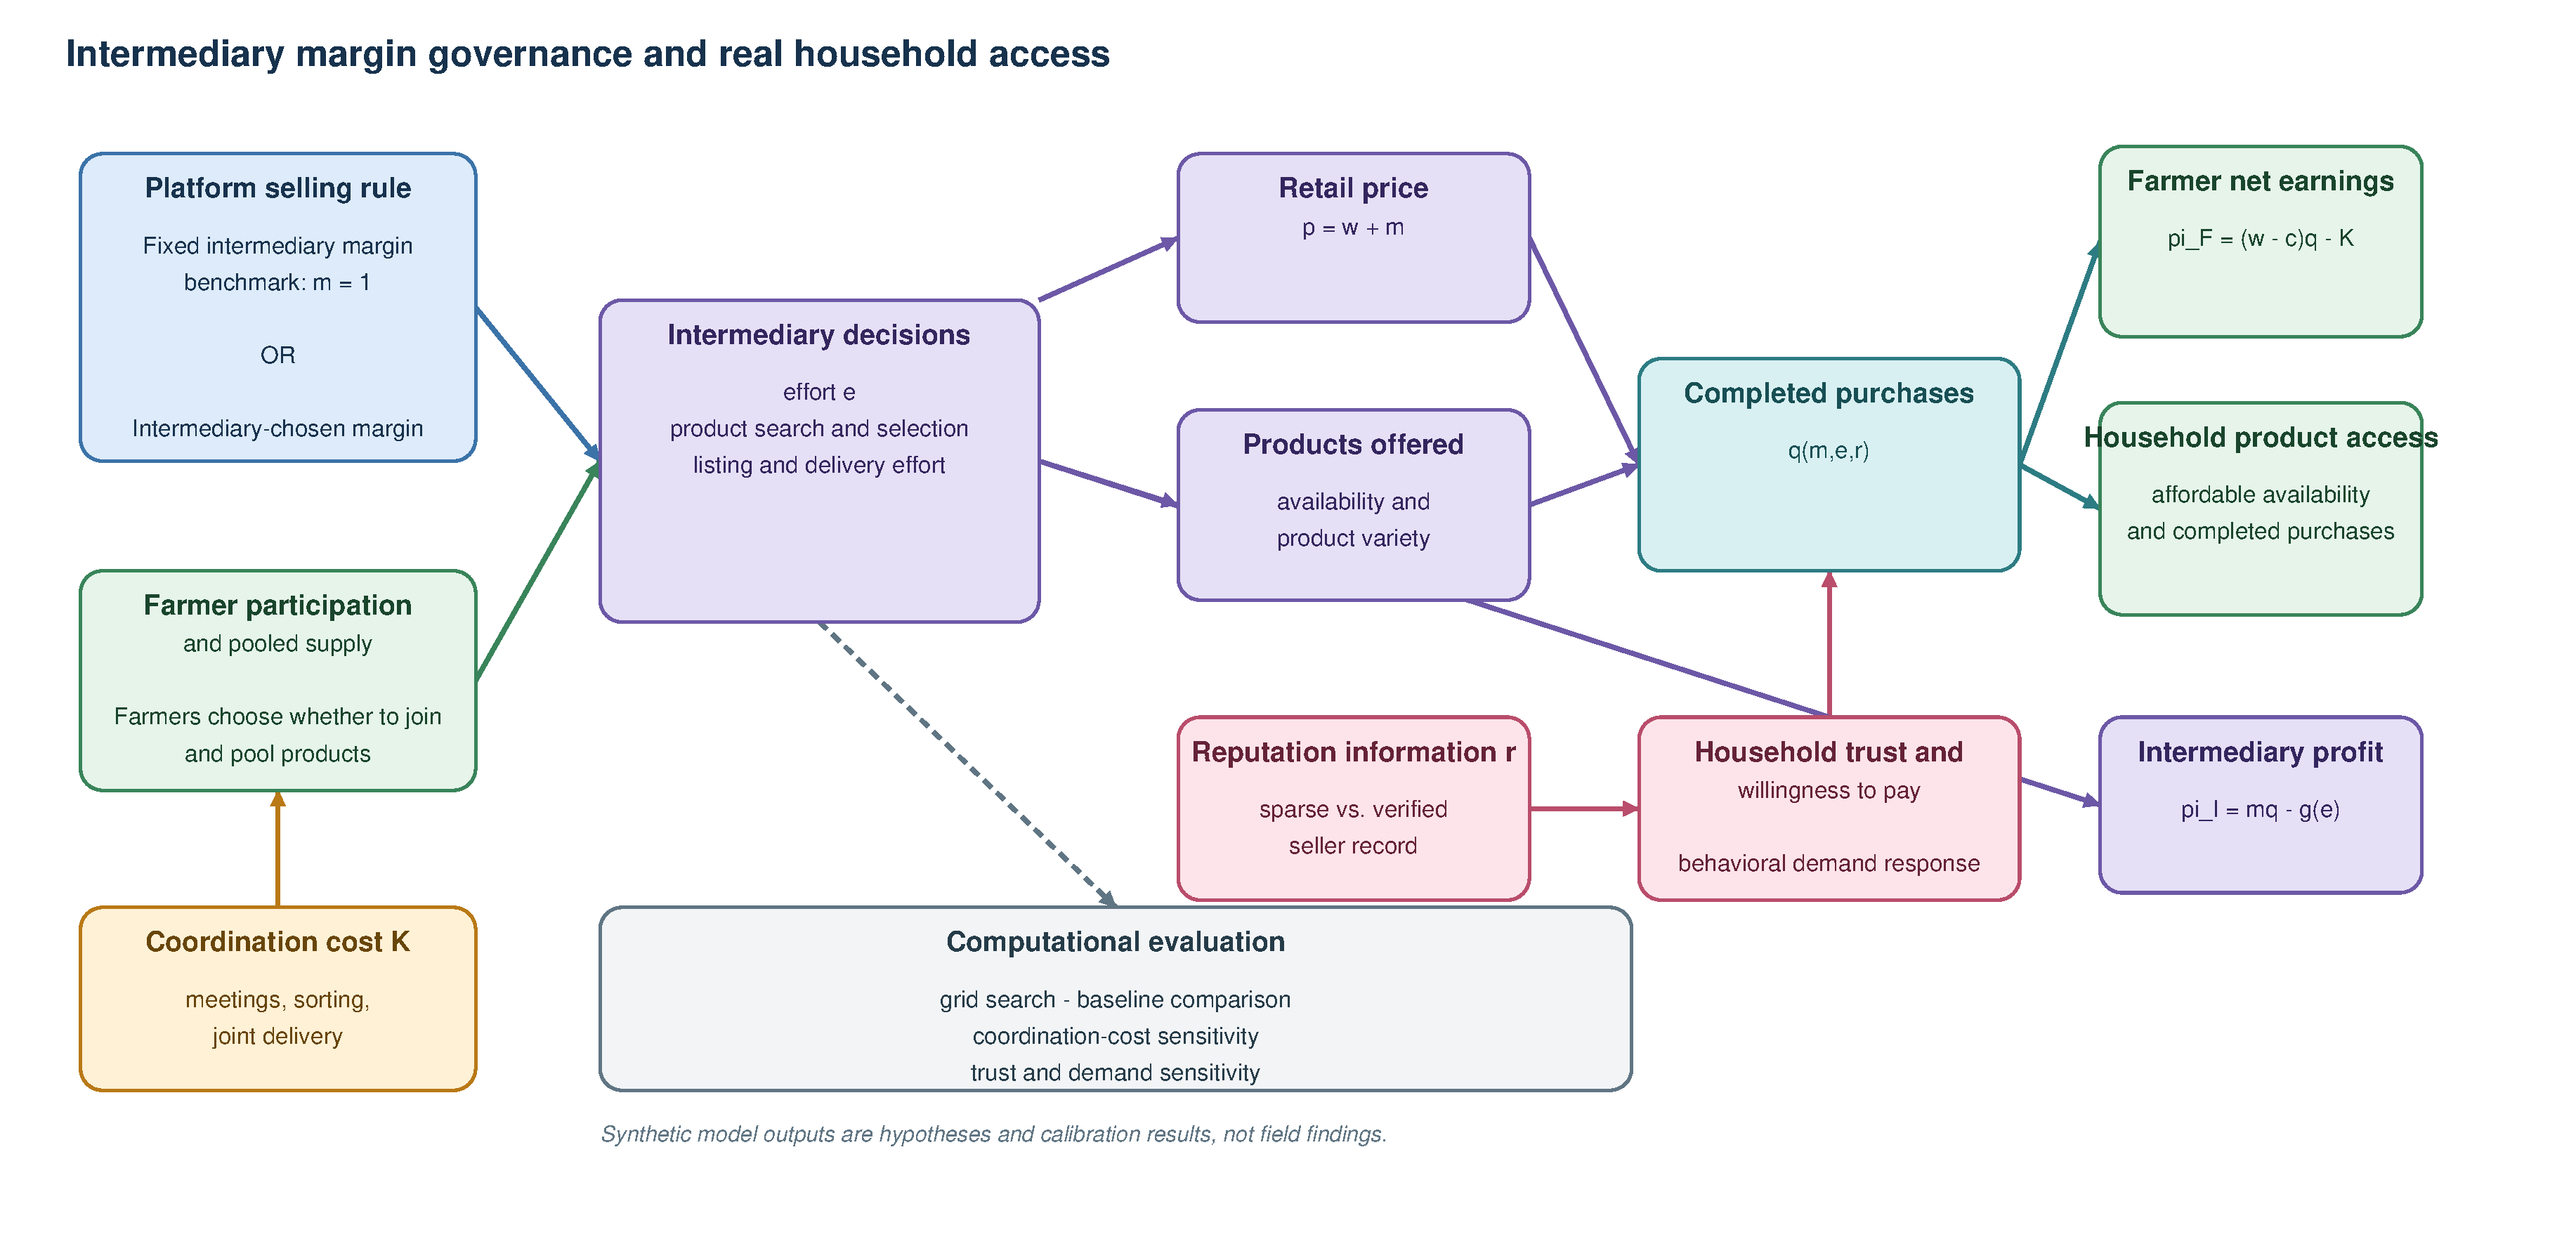
\includegraphics[width=\textwidth]{figures/ps1_teaser.pdf}
\caption{Proposed causal chain. A platform sets a fixed margin or lets an intermediary choose it. The rule changes intermediary effort and product selection, which affect retail prices, completed purchases, and farmers' net earnings after coordination costs. Reputation information changes household trust and willingness to buy. Arrows are hypotheses, not observed causal effects.}
\Description{An editable flow diagram compares fixed and chosen intermediary margins, effort and product selection, retail price and completed purchases, farmer net earnings, household access, and reputation-based trust.}\label{fig:teaser}\end{teaserfigure}
\maketitle\raggedbottom
\noindent\textbf{COMSCI/ECON 206 --- Computational Microeconomics.} Autumn 2026 Session 1. Group 1 -- Economist. Instructor: Prof. Luyao Zhang. PS1 research proposal.\par\smallskip
\section{Three connected research questions}
Small farmers may pool products and sell through an intermediary who reaches households in underserved markets. The arrangement reduces search costs, but the intermediary's margin rule divides surplus and shapes effort and product selection. Coase explains why transaction costs shape organization~\cite{coase1937,nobelcoase1991}. Morgenstern et al. show that resale-platform margin competition can reduce product-search effort and that centralized margin decisions shift competition toward product selection~\cite{morgenstern2025}. I adapt this mechanism to farmer sales; their paper does not establish rural-consumption-inequality effects.

\textbf{Q1---Economics:} How do fixed and intermediary-chosen margins affect farmer net earnings and household product access when effort and coordination costs matter?\\
\textbf{Q2---Computation:} Under which demand, cost, competition, and trust conditions does each rule improve participation, completed purchases, and surplus?\\
\textbf{Q3---Behavior:} Does reputation information raise trust and willingness to pay enough to change which rule performs better?\\
\textbf{Integrated question:} Which rule improves farmer earnings and real household access after effort, product selection, coordination cost, and trust are included? Figure~\ref{fig:teaser} displays the causal chain.

\section{Answer to the economics question}
The players are a platform, a pooled farmer group, an intermediary, and households. The platform selects $R\in\{F,C\}$; farmers choose participation and pay coordination cost $K$; under $F$ the platform fixes margin $m$, while under $C$ the intermediary chooses $m$ and effort $e$. Let $w$ be the farmer payment, $c$ unit cost, $p=w+m$, and $q(m,e,r)$ completed purchases, with $r$ a reputation signal. Payoffs are
\[\pi_F=(w-c)q-K,\qquad \pi_I=mq-g(e).\]
I solve this sequential game by backward induction. The testable prediction is a tradeoff: a moderate fixed margin can lower retail price and raise purchases, while a chosen margin can increase intermediary profit and effort; very low margins may cause exit. This is a hypothesis, not an assumed benefit of collective selling.

\section{Answer to the computational question}
The notebook implements a computational grid search. It searches feasible $(m,e)$ choices, applies farmer participation, and reports price, completed quantity, farmer earnings, intermediary profit, and surplus. With $q=12e\max\{0,4-m\}$, $w=6$, $c=4$, $K=12$, $g(e)=30e^2$, and fixed $m=1$, the synthetic baseline gives fixed $(e,q,\pi_F)=(0.60,21.60,31.20)$. The chosen-margin grid gives $(m,e,q,\pi_F)=(2.00,0.80,19.20,26.40)$ and intermediary profit $19.20$ versus $10.80$ under the fixed rule. These are synthetic outputs, not field findings. Sensitivity analysis varies coordination cost, demand, trust, effort cost, competition, and heterogeneous products; variety is a planned extension.

\clearpage\balance
\section{Answer to the behavioral question}
Households may not convert listed availability into purchases if they distrust an unfamiliar seller. Building on reputation experiments~\cite{resnick2006} and bounded rationality~\cite{simon1955}, I will estimate purchase probability at a given posted price under sparse versus verified reputation information. Purchase, trust, and willingness-to-pay measures distinguish a trust mechanism from a price-only explanation. The estimated response replaces $r$ in $q(m,e,r)$ and the simulation is rerun. A small online study cannot identify long-run farmer income or population welfare; a result showing no reputation effect or a consistent advantage for chosen margins would revise my hypothesis.

\section{Advanced development and future directions}
This proposal extends Coase's transaction-cost question~\cite{coase1937,nobelcoase1991} to digital intermediation between farmers and underserved households. Newell and Simon's Turing-recognized work on computational decision processes~\cite{turing1975} motivates an inspectable model of bounded choices. Today's platforms can jointly set margins, rank products, and display reputation. Current resale-platform theory does not determine whether these rules raise farmer earnings after coordination costs or turn listed products into trusted completed purchases.
\begin{table}[h]\caption{Roadmap from foundation to contribution.}\begin{tabularx}{\columnwidth}{@{}p{1.25cm}Y@{}}\toprule\textbf{Stage}&\textbf{Milestone}\\\midrule Foundation&Coase on organization; Newell and Simon on computational decisions.\\ PS1&Fixed/chosen margin baseline with coordination cost.\\ Next&Trust evidence, product heterogeneity, competition, and field validation.\\ 2056&Adaptive, auditable rules that improve access and producer welfare.\\\bottomrule\end{tabularx}\end{table}
\noindent\textbf{Expected 2056 Nobel Prize and Turing Award contribution statement.} By 2056, I aspire to develop a general theory and open computational system for designing intermediated markets under transaction costs and bounded trust. I will connect economic incentives, auditable simulation, and behavioral evidence to identify rules that improve access without weakening producer participation.
\subsection*{Open Science Statement}\textbf{GitHub:} \GitHubLink\\\textbf{Colab:} \ColabLink\\\textbf{Submitted commit:} \SubmittedCommit\\The repository contains the model, requirements, notebook, tests, synthetic inputs, and saved outputs. A clean run reproduces the baseline and sensitivity files.
\subsection*{Statement of Contribution to the UN's SDGs}\textbf{Hugging Face:} \DemoLink\\The planned Margin Rule Lab will support \textbf{SDG 4---Quality Education}~\cite{sdg4} by letting learners vary margins, coordination costs, effort costs, and reputation and observe synthetic access and earnings outcomes. Educational benefit will be checked with a short pre/post question.
\clearpage\nobalance
\section*{Author Notes}
\subsection*{Acknowledgements}
I thank Prof. Luyao Zhang, Program Chair, Prof. Ken Rogerson, Program Discussant, Jiayang [SURNAME], Xuantong [SURNAME], and the COMSCI/ECON 206 Autumn 2026 Session 1 class. Jiayang's reputation discussion motivated the behavioral demand condition; Xuantong's rule-comparison discussion motivated completed access as an outcome. Prof. Zhang's feedback led me to compare fixed and chosen intermediary margins and include coordination costs. I am responsible for the proposal, code, and remaining errors.
\subsection*{Individual contribution}
I designed the farmer-intermediary application, sequential model, synthetic baseline, computational checks, and proposed reputation test. I wrote and verified the code and adapted the cited theories and class feedback with acknowledgement.
\bibliographystyle{ACM-Reference-Format}\bibliography{references}
\appendix
\section{Technical details and reproducibility}
The baseline uses $q(m,e)=12e\max\{0,4-m\}$, $g(e)=30e^2$, $w=6$, $c=4$, and $K=12$. Fixed $m=1$; chosen searches $m\in[0,4]$ by $0.05$ and $e\in[0,1]$ by $0.01$. The committed notebook and `companion/outputs/` reproduce the values in Section 3. All results are synthetic.
\subsection{AI-use disclosure}
OpenAI GPT-6 assisted with drafting, debugging, documentation, and consistency checks on September 13, 2026 after I selected the question and supplied course feedback. I verified equations, outputs, citations, and scope. Initial reasoning, handwritten reflection, and peer reviews are Human-Only.
\section{Cumulative Intellectual Development}
This proposal develops Intellectual Statements I and II through the \emph{2056 Nobel and Turing Laureate Program Launch Workshop}, September 7, 2026, Duke Kunshan University, IB 2050. My session was Group 1 and my role was economist. My first statement asked whether price information could strengthen farmers' bargaining positions. Week 2 shifted the mechanism toward pooled selling and organization. Prof. Zhang then specified one chain from selling rule to household opportunity: compare fixed and chosen margins and include coordination costs. I retained the bargaining concern but replaced broad transparency and inequality claims with measurable farmer earnings and completed household purchases.
\section{Field and open-source inspiration}
The \emph{Joint Interdisciplinary Field Trip---Technology, Computation, Culture \& Society in Action} occurred September 4, 2026. I attended the Tencent Shanghai Office and Shanghai Science and Technology Museum visits. Retain the two existing photographs with exact date and provenance in the figure captions; distinguish observation from interpretation. Open Food Network motivates coordinated producer listings~\cite{openfoodnetwork}; CKAN motivates publishing parameters and outputs~\cite{ckan}. These sources inspire the design but are not causal evidence for farmer earnings.
\section{Review response and revision record}
Peer review, rebuttal, reviewer follow-up, and v2 will be completed in the Human-Only class process. Preserve v1, both reviews, the response, follow-up, and v2 here; do not place private review documents in the public GitHub repository.
\clearpage\onecolumn
\section{Structured abstract and cumulative proposal map}\label{app:abstract}
\begin{table}[H]\caption{Appendix E: eight-row structured abstract.}\renewcommand{\arraystretch}{1.15}\begin{tabularx}{\textwidth}{@{}p{.25\textwidth}Y@{}}\toprule\textbf{Element}&\textbf{Current statement}\\\midrule
Background&Small farmers can pool products and use intermediaries to reach underserved households; margin and selection rules affect effort, prices, and surplus.\\
Motivation and application&A platform or cooperative must choose how an intermediary earns a margin without reducing farmer participation or completed household purchases.\\
Three connected questions&Economics compares rules; computation finds thresholds; behavioral science estimates how reputation changes trust and demand.\\
Method and model assumptions&Sequential game with farmer coordination cost, intermediary margin and effort, household purchase, grid search, sensitivity analysis, and a reputation experiment.\\
Results or expected results&Current synthetic baseline favors fixed margins for farmer earnings and completed units, while chosen margins favor intermediary profit; reversals remain expected under other parameters.\\
Intellectual merits&The project identifies the mechanism linking margin governance, coordination cost, computational thresholds, and trust.\\
Practical impacts&Platforms can compare rules before implementation; the Margin Rule Lab will teach the tradeoff for SDG 4.\\
Feedback received and revision made&Prof. Zhang recommended fixed versus chosen margins, coordination costs, and one chain to household opportunity. I replaced broad inequality claims with this bounded mechanism.\\\bottomrule\end{tabularx}\end{table}
\end{document}
